\documentclass[conference]{IEEEtran}
\usepackage{graphicx}
\usepackage{amsmath}
\usepackage{amssymb}
\usepackage{booktabs}
\usepackage{multirow}
\usepackage{url}
\usepackage{cite}
\usepackage{microtype}

\begin{document}

\title{Manual Dropout in Neural Networks:\\A Reduced-Scale Reproduction and Ablation Study}

\author{
  \IEEEauthorblockN{STUDENT\_NAME\_PENDING}
  \IEEEauthorblockA{Roll No. 24CS2032\\
  Course Implementation Study\\
  Deep Learning (24CS2032)}
}

\maketitle

\begin{abstract}
Dropout regularizes deep neural networks by stochastically omitting hidden units during training to suppress feature co-adaptation. In this study, we implement inverted dropout from first principles in PyTorch without built-in library modules. We conduct a fixed-budget rate ablation across eight drop rates ($d \in \{0.0, 0.1, 0.2, 0.3, 0.4, 0.5, 0.6, 0.7\}$) across three seeds ($42, 43, 44$) on a three-hidden-layer MLP ($784 \to 256 \to 256 \to 256 \to 10$). On MNIST, mean validation error selects $d=0.4$, lowering test error from $4.320 \pm 0.295\%$ to $3.843 \pm 0.282\%$ ($11.03\%$ relative error reduction). On the Fashion-MNIST extension using the same protocol, validation error selects $d=0.2$, reducing test error from $14.663 \pm 0.175\%$ to $14.347 \pm 0.253\%$ ($2.16\%$ relative reduction). Conversely, higher rates degrade performance under the fixed 20-epoch budget. Under our reduced-scale experimental constraints, dropout provides measurable regularization, with optimal rates depending on dataset characteristics and requiring validation-based selection.
\end{abstract}

\begin{IEEEkeywords}
Dropout, regularization, neural networks, ablation study, model selection, MNIST, Fashion-MNIST.
\end{IEEEkeywords}

\section{Introduction}
Deep neural networks possess remarkable expressive capacity, enabling them to approximate complex non-linear functions. However, when parameter capacity is large relative to the volume of training examples, networks readily memorize training noise and overfit, yielding high generalization error on unseen test data~\cite{srivastava2014dropout}.

To mitigate overfitting, ensemble methods combine predictions from multiple independently trained models. While effective, training and maintaining large ensembles of deep neural networks is computationally prohibitive. In their seminal work, Srivastava et al.~\cite{srivastava2014dropout} introduced dropout as a computationally efficient approximation to model ensembling. By stochastically dropping units during each training iteration, dropout trains an exponential family of thinned subnetworks that share weights, creating an implicit geometric ensemble at evaluation time.

The objective of this assignment is to implement dropout from first principles using Python and PyTorch without relying on built-in primitives such as \texttt{torch.nn.Dropout} or \texttt{torch.nn.functional.dropout}. We evaluate this manual implementation through a controlled drop-rate ablation across eight uniform rates ($d \in \{0.0, 0.1, 0.2, 0.3, 0.4, 0.5, 0.6, 0.7\}$) using three fixed initialization seeds ($42, 43, 44$). We investigate both the primary MNIST handwritten digit benchmark~\cite{lecun1998mnist} and an identical-protocol extension to Fashion-MNIST~\cite{xiao2017fashion}.

We emphasize that this project is an educational, reduced-scale reproduction rather than an attempt to replicate the exact state-of-the-art numerical accuracies of the original 2014 publication. We employ a fixed parameter width, a sub-sampled training set of 10,000 examples, and a constrained budget of 20 training epochs. Crucially, we adhere to strict scientific evaluation: hyperparameters and drop rates are chosen exclusively on validation data, leaving the official test set for unbiased descriptive evaluation. Our empirical findings demonstrate that while dropout yields noticeable error reductions at moderate rates, high dropout rates degrade generalization under fixed compute budgets, confirming that regularization strength must be calibrated carefully.

\section{Dropout Formulation and Architecture}

\subsection{Mathematical Formulation}
Let $h \in \mathbb{R}^D$ denote the post-activation vector of a hidden neural network layer. We define the drop probability as $d \in [0, 1)$ and the corresponding retention or keep probability as:
\begin{equation}
q = 1 - d, \quad q \in (0, 1].
\end{equation}
During training, a random binary mask vector $m \in \{0, 1\}^D$ is sampled independently across units from a Bernoulli distribution parameterized by $q$:
\begin{equation}
m_i \sim \text{Bernoulli}(q), \quad \mathbb{P}(m_i = 1) = q, \quad \mathbb{P}(m_i = 0) = d.
\end{equation}

In modern deep learning implementations, inverted dropout is the standard formulation. Rather than scaling activations at test time, inverted dropout rescales the unmasked activations during training by the reciprocal of the keep probability, $1/q$:
\begin{equation}
\tilde{h}_i^{(\text{train})} = \frac{m_i \cdot h_i}{q}.
\end{equation}
During evaluation (inference), the dropout operator is entirely bypassed:
\begin{equation}
\tilde{h}_i^{(\text{eval})} = h_i.
\end{equation}

\subsection{Expectation Derivation}
The primary mathematical justification for the $1/q$ scaling factor is preservation of the expected activation magnitude across training and evaluation phases. For any arbitrary unit activation $h_i$, the conditional expectation of $\tilde{h}_i^{(\text{train})}$ given $h_i$ is derived as follows:
\begin{align}
\mathbb{E}\left[\tilde{h}_i^{(\text{train})} \mid h_i\right] &= \mathbb{E}\left[\frac{m_i \cdot h_i}{q} \;\middle|\; h_i\right] \\
&= \frac{h_i}{q} \, \mathbb{E}\left[m_i\right] \\
&= \frac{h_i}{q} \cdot \left(1 \cdot \mathbb{P}(m_i=1) + 0 \cdot \mathbb{P}(m_i=0)\right) \\
&= \frac{h_i}{q} \cdot q \\
&= h_i.
\end{align}
Because $\mathbb{E}\left[\tilde{h}_i^{(\text{train})} \mid h_i\right] = \tilde{h}_i^{(\text{eval})} = h_i$, the input distribution received by subsequent downstream layers maintains an identical expected mean during training and evaluation. Consequently, downstream weights do not require post-hoc rescaling at inference time, ensuring that evaluation mode remains entirely deterministic and computationally identical to an unregularized forward pass.

\subsection{Inverted Dropout vs. Original Paper Formulation}
In the original presentation by Srivastava et al.~\cite{srivastava2014dropout}, dropout was formulated using standard test-time scaling: during training, activations were unscaled ($\tilde{h}_i = m_i \cdot h_i$), and at test time, outgoing weights or activations were multiplied by the keep probability ($\tilde{h}_i = q \cdot h_i$). Reference materials on the author's project page~\cite{srivastava2014dropoutpage} and the historical Deepnet repository~\cite{srivastava2014deepnet} document this classical convention.

Both conventions are mathematically equivalent in expectation, as both maintain identical forward signal magnitudes across phases. Inverted dropout is widely preferred in modern production frameworks (such as PyTorch~\cite{pytorch_dropout}) because it restricts stochasticity and scaling logic entirely to the training graph. At inference time, no extra arithmetic operations or memory allocations are introduced.

\subsection{Network Architecture}
All experiments employ a Multilayer Perceptron (MLP) consisting of three fully connected hidden layers:
\begin{align}
\mathbf{x} \in \mathbb{R}^{784} &\xrightarrow{W_1, b_1} \mathbb{R}^{256} \xrightarrow{W_2, b_2} \mathbb{R}^{256} \nonumber \\
&\xrightarrow{W_3, b_3} \mathbb{R}^{256} \xrightarrow{W_4, b_4} \mathbf{y} \in \mathbb{R}^{10}.
\end{align}
Each linear hidden layer is followed by a Rectified Linear Unit (ReLU) activation function:
\begin{equation}
\sigma(z) = \max(0, z).
\end{equation}
Our custom \texttt{ManualDropout} layer is inserted immediately after each hidden ReLU activation. In strict accordance with the project specification:
\begin{itemize}
\item No dropout is applied to the raw input layer ($d_{\text{in}} = 0$).
\item No dropout is applied to the final classification logits.
\item Built-in dropout routines (\texttt{torch.nn.Dropout}) are strictly forbidden.
\item The total trainable parameter count is exactly:
\begin{align}
(784 \times 256 + 256) &+ 2 \times (256 \times 256 + 256) \nonumber \\
&+ (256 \times 10 + 10) = 335{,}114.
\end{align}
\end{itemize}

\section{Experimental Setup}

\subsection{Protocol Specification (\texttt{dropout-24cs2032-v1})}
We freeze the experimental configuration under protocol identifier \texttt{dropout-24cs2032-v1}. Key experimental parameters are detailed in Table~\ref{tab:protocol}.

\begin{table}[htbp]
\caption{Frozen Experimental Protocol Parameters}
\label{tab:protocol}
\centering
\setlength{\tabcolsep}{4pt}
\begin{tabular}{ll}
\toprule
\textbf{Parameter} & \textbf{Specification} \\
\midrule
Architecture & $784 \to 256 \to 256 \to 256 \to 10$ MLP \\
Hidden Activation & Rectified Linear Unit (ReLU) \\
Dropout Placement & After hidden ReLUs (Layers 1, 2, 3) \\
Drop Rates ($d$) & $0.0, 0.1, 0.2, 0.3, 0.4, 0.5, 0.6, 0.7$ \\
Keep Rates ($q$) & $1.0, 0.9, 0.8, 0.7, 0.6, 0.5, 0.4, 0.3$ \\
Initialization Seeds & $42, 43, 44$ (3 seeds) \\
Split Seed & $2026$ \\
Training Set Size & $10{,}000$ examples (disjoint subset) \\
Validation Set Size & $5{,}000$ examples (disjoint subset) \\
Test Set Size & $10{,}000$ examples (official test split) \\
Training Epochs & $20$ fixed epochs \\
Mini-Batch Size & $128$ \\
Optimizer & Adam ($\beta_1=0.9, \beta_2=0.999$, $\epsilon=10^{-8}$) \\
Learning Rate & $0.001$ (fixed, no decay schedule) \\
Weight Decay & $0.0$ (no $L_2$ regularization) \\
Other Regularizers & None (no batch norm, no max-norm) \\
Data Preprocessing & Division by $255.0$ (float32 scaling) \\
Compute Backend & CPU (Apple Silicon arm64, native) \\
\bottomrule
\end{tabular}
\end{table}

\subsection{Data Partitioning and Fair Initialization}
The official torchvision datasets~\cite{torchvision_mnist, torchvision_fashion} provide 60,000 training and 10,000 test images. To operate within a standardized educational compute budget, we fix split seed $2026$ to partition the 60,000 training images into 10,000 training examples, 5,000 validation examples, and 45,000 unused images. The official 10,000 test images remain completely untouched and are reserved exclusively for final evaluation.

To ensure strict experimental fairness across drop rates, we enforce deterministic initialization: for any given random seed ($s \in \{42, 43, 44\}$), the model weights across all eight drop rates ($d \in [0.0, 0.7]$) are verified to be bitwise identical at step 0 before optimization begins.

\subsection{Model Selection and Evaluation Policy}
Model selection is governed strictly by minimum validation error:
\begin{equation}
d^* = \arg\min_{d} \; \overline{\text{Error}}_{\text{val}}(d),
\end{equation}
where $\overline{\text{Error}}_{\text{val}}(d)$ is the mean classification error across the three seeds at epoch 20. Ties are resolved by selecting the lower drop rate. 

In strict adherence to sound scientific methodology, test set performance is never consulted during rate selection, checkpoint picking, or hyperparameter adjustment. All reported test errors are unbiased descriptive metrics evaluated at the fixed termination epoch ($E=20$). Statistical dispersion is reported using the sample standard deviation ($ddof=1$).

\subsection{Hardware and Execution Environment}
Experiments were executed on macOS 26.6.2 (Darwin arm64) using Python 3.13.9, PyTorch 2.14.1, torchvision 0.29.1, and NumPy 2.5.3. Preliminary benchmarks revealed that CPU execution required 0.785 seconds per 2-epoch run compared to 4.398 seconds on Apple Metal Performance Shaders (MPS), representing an efficiency advantage of over $5.5\times$ for CPU. This performance difference is attributed to GPU kernel launch and synchronization latency on small parameter tensors (335k parameters). Consequently, CPU was locked as the deterministic compute backend.

\section{Experimental Results}

\subsection{MNIST Main Reproduction}
The complete sweep of 24 independent runs (8 rates $\times$ 3 seeds) was executed to fixed epoch 20. Table~\ref{tab:mnist_summary} details the training, validation, and test error rates across all evaluated drop rates.

\begin{table}[htbp]
\caption{MNIST Results at Epoch 20 (Mean $\pm$ SD over Seeds 42, 43, 44)}
\label{tab:mnist_summary}
\centering
\setlength{\tabcolsep}{2.2pt}
\begin{tabular}{cccc}
\toprule
\textbf{Rate ($d$)} & \textbf{Train Error (\%)} & \textbf{Val Error (\%)} & \textbf{Test Error (\%)} \\
\midrule
$0.0$ (Baseline) & $0.203 \pm 0.200$ & $4.260 \pm 0.533$ & $4.320 \pm 0.295$ \\
$0.1$ & $0.090 \pm 0.044$ & $4.180 \pm 0.314$ & $4.050 \pm 0.278$ \\
$0.2$ & $0.110 \pm 0.000$ & $3.893 \pm 0.099$ & $3.900 \pm 0.239$ \\
$0.3$ & $0.240 \pm 0.080$ & $3.753 \pm 0.061$ & $3.820 \pm 0.118$ \\
\textbf{0.4 (Selected)} & $\mathbf{0.323 \pm 0.047}$ & $\mathbf{3.747 \pm 0.130}$ & $\mathbf{3.843 \pm 0.282}$ \\
$0.5$ (Reference) & $0.700 \pm 0.044$ & $3.840 \pm 0.140$ & $3.883 \pm 0.087$ \\
$0.6$ & $1.273 \pm 0.057$ & $4.407 \pm 0.219$ & $4.380 \pm 0.104$ \\
$0.7$ & $2.513 \pm 0.153$ & $5.133 \pm 0.090$ & $5.110 \pm 0.147$ \\
\bottomrule
\end{tabular}
\end{table}

\textbf{Baseline Performance:} The unregularized baseline ($d=0.0$) achieves a training error of $0.203 \pm 0.200\%$, validation error of $4.260 \pm 0.533\%$, and test error of $4.320 \pm 0.295\%$, representing a substantial generalization gap of $4.117 \pm 0.101$ percentage points (pp).

\textbf{Validation-Selected Model:} The lowest mean validation error is attained at drop rate $d=0.4$ ($3.747 \pm 0.130\%$). At this rate, the model achieves a test error of $3.843 \pm 0.282\%$ (accuracy: $96.157\%$). Compared to the unregularized baseline, $d=0.4$ yields an absolute reduction in test error of $0.477$ pp, corresponding to a relative test error reduction of:
\begin{equation}
\frac{4.320 - 3.843}{4.320} \times 100\% = 11.03\%.
\end{equation}
Furthermore, the generalization gap narrows from $4.117$ pp to $3.520 \pm 0.295$ pp.

\textbf{Test Set Nuance:} Descriptively, the lowest numerical test error was observed at $d=0.3$ ($3.820 \pm 0.118\%$). However, because model selection is strictly confined to validation data, $d=0.4$ remains the sole authorized selected model. The difference between test error at $d=0.3$ ($3.820\%$) and $d=0.4$ ($3.843\%$) is minor ($0.023$ pp) and falls well within the sample standard deviation ($0.282\%$).

\textbf{Negative Findings:} When the drop rate is increased to $d=0.6$ and $d=0.7$, test performance deteriorates to $4.380 \pm 0.104\%$ and $5.110 \pm 0.147\%$ respectively, both performing markedly worse than the unregularized baseline.

\subsection{Fashion-MNIST Extension}
To evaluate whether these regularizing properties generalize beyond digit recognition, we executed the identical 24-run protocol on Fashion-MNIST~\cite{xiao2017fashion} as an extension using the same experimental protocol. Table~\ref{tab:fashion_summary} summarizes the results.

\begin{table}[htbp]
\caption{Fashion-MNIST Results at Epoch 20 (Mean $\pm$ SD over Seeds 42, 43, 44)}
\label{tab:fashion_summary}
\centering
\setlength{\tabcolsep}{2.2pt}
\begin{tabular}{cccc}
\toprule
\textbf{Rate ($d$)} & \textbf{Train Error (\%)} & \textbf{Val Error (\%)} & \textbf{Test Error (\%)} \\
\midrule
$0.0$ (Baseline) & $7.130 \pm 0.177$ & $13.127 \pm 0.247$ & $14.663 \pm 0.175$ \\
$0.1$ & $7.587 \pm 0.471$ & $13.113 \pm 0.042$ & $14.220 \pm 0.105$ \\
\textbf{0.2 (Selected)} & $\mathbf{8.583 \pm 0.414}$ & $\mathbf{13.087 \pm 0.408}$ & $\mathbf{14.347 \pm 0.253}$ \\
$0.3$ & $9.393 \pm 0.067$ & $13.267 \pm 0.244$ & $14.567 \pm 0.396$ \\
$0.4$ & $10.060 \pm 0.584$ & $13.573 \pm 0.494$ & $14.647 \pm 0.330$ \\
$0.5$ (Reference) & $10.990 \pm 0.366$ & $13.747 \pm 0.200$ & $15.133 \pm 0.325$ \\
$0.6$ & $12.273 \pm 0.323$ & $14.380 \pm 0.053$ & $15.730 \pm 0.373$ \\
$0.7$ & $14.543 \pm 0.468$ & $15.673 \pm 0.380$ & $17.453 \pm 0.376$ \\
\bottomrule
\end{tabular}
\end{table}

\textbf{Baseline Performance:} The unregularized baseline ($d=0.0$) produces a training error of $7.130 \pm 0.177\%$, validation error of $13.127 \pm 0.247\%$, and test error of $14.663 \pm 0.175\%$ with a generalization gap of $7.533 \pm 0.351$ pp.

\textbf{Validation-Selected Model:} Validation error selects drop rate $d=0.2$ ($13.087 \pm 0.408\%$). The selected model attains a test error of $14.347 \pm 0.253\%$ (accuracy: $85.653\%$), yielding an absolute reduction of $0.317$ pp ($2.16\%$ relative reduction) and contracting the generalization gap to $5.763 \pm 0.165$ pp.

\textbf{Critical Negative Finding:} Notably, the standard paper reference rate of $d=0.5$ yields a test error of $15.133 \pm 0.325\%$, which is $0.470$ pp \emph{worse} than the no-dropout baseline. At $d=0.7$, test error degrades sharply to $17.453 \pm 0.376\%$. This highlights that applying a canonical drop rate of $d=0.5$ without validation tuning can actively harm model accuracy on more complex visual benchmarks.

\subsection{Learning Dynamics and Overfitting}
Figure~\ref{fig:overfitting} illustrates the epoch-wise training error, test error, and validation loss trajectories on MNIST for the baseline ($d=0.0$) and reference dropout ($d=0.5$).

\begin{figure}[htbp]
\centering
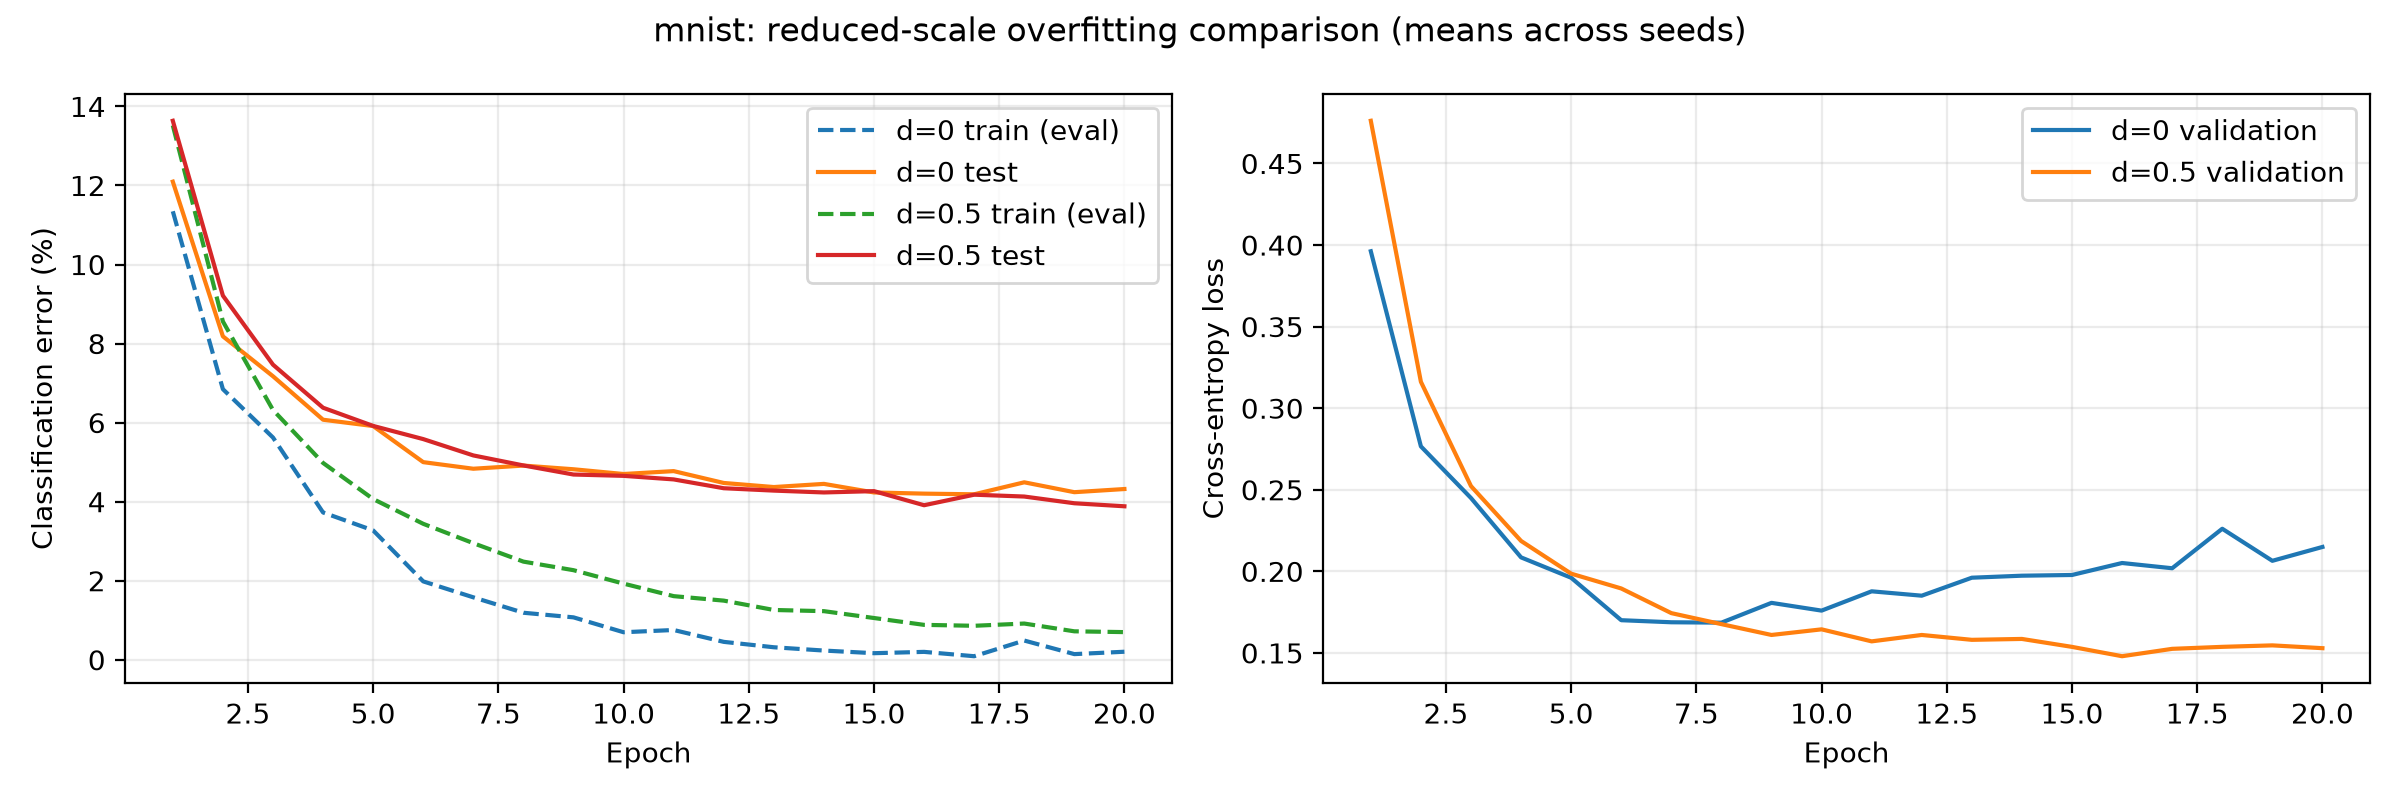
\includegraphics[width=0.80\columnwidth]{figures/mnist_overfitting.png}
\caption{Epoch-wise learning dynamics on MNIST comparing unregularized training ($d=0.0$) against dropout ($d=0.5$) under our reduced-scale protocol ($10{,}000$ training examples, $20$ epochs). While the unregularized model drives training error toward zero and exhibits rising validation loss (overfitting), dropout regularizes the representation, maintaining stable validation loss and lower test error.}
\label{fig:overfitting}
\end{figure}

In the baseline model ($d=0.0$), training error rapidly declines toward $0.2\%$, while validation loss diverges after epoch 6, evidencing severe memorization. In contrast, with dropout enabled ($d=0.5$), training error declines more gradually, and validation loss stabilizes at a lower plateau, illustrating effective regularization of network capacity.

\subsection{Keep-Probability Ablation Curves}
Figure~\ref{fig:keep_prob_mnist} and Figure~\ref{fig:keep_prob_fashion} present the relationships between test error and keep probability $q = 1 - d$ for MNIST and Fashion-MNIST respectively.

\begin{figure*}[t]
\centering
\begin{minipage}[b]{0.48\textwidth}
\centering
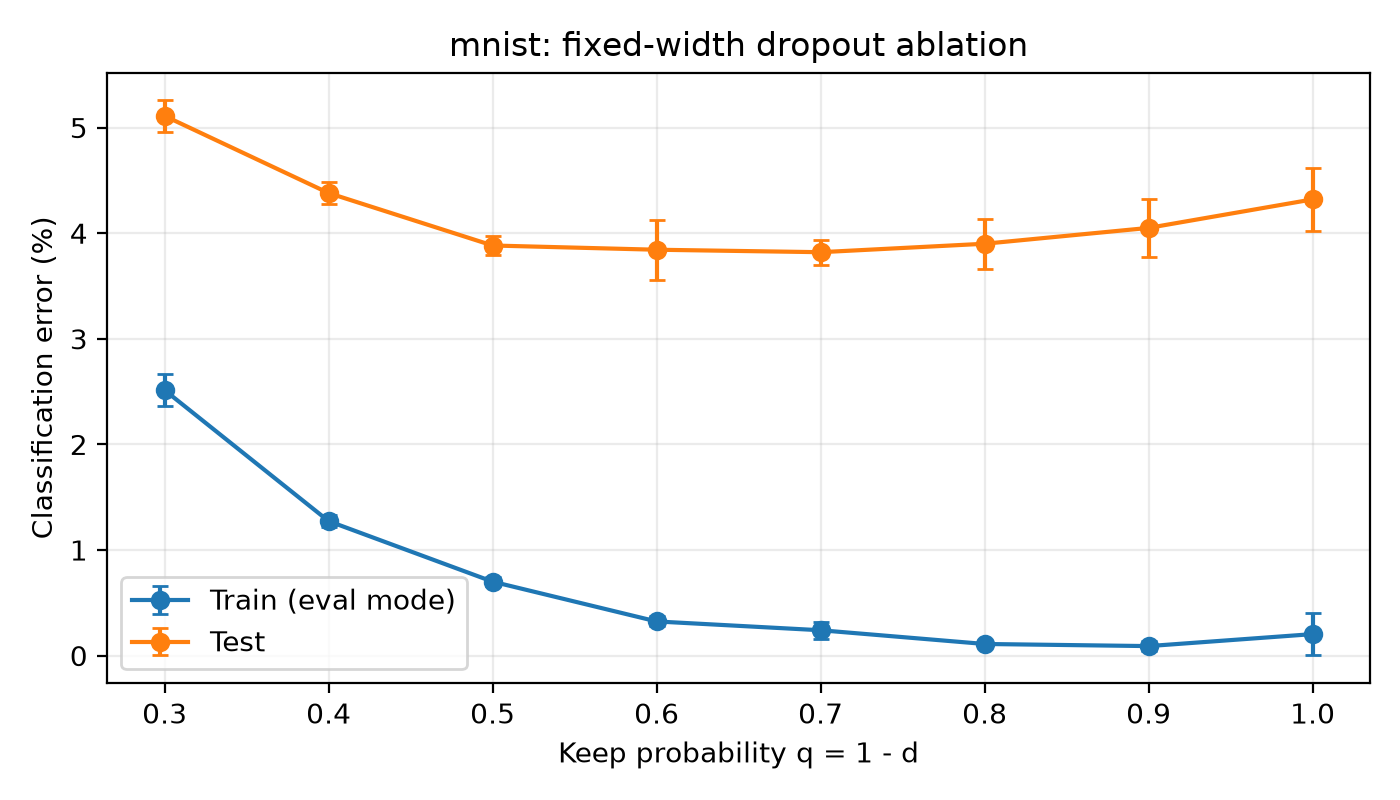
\includegraphics[width=0.78\linewidth]{figures/mnist_keep_probability.png}
\caption{Reduced-scale fixed-width dropout rate ablation on MNIST inspired by Srivastava et al.~\cite{srivastava2014dropout}, Fig.~9(a). Data points depict measured experimental results (mean $\pm$ sample SD across three seeds) plotted against keep probability $q = 1 - d$.}
\label{fig:keep_prob_mnist}
\end{minipage}
\hfill
\begin{minipage}[b]{0.48\textwidth}
\centering
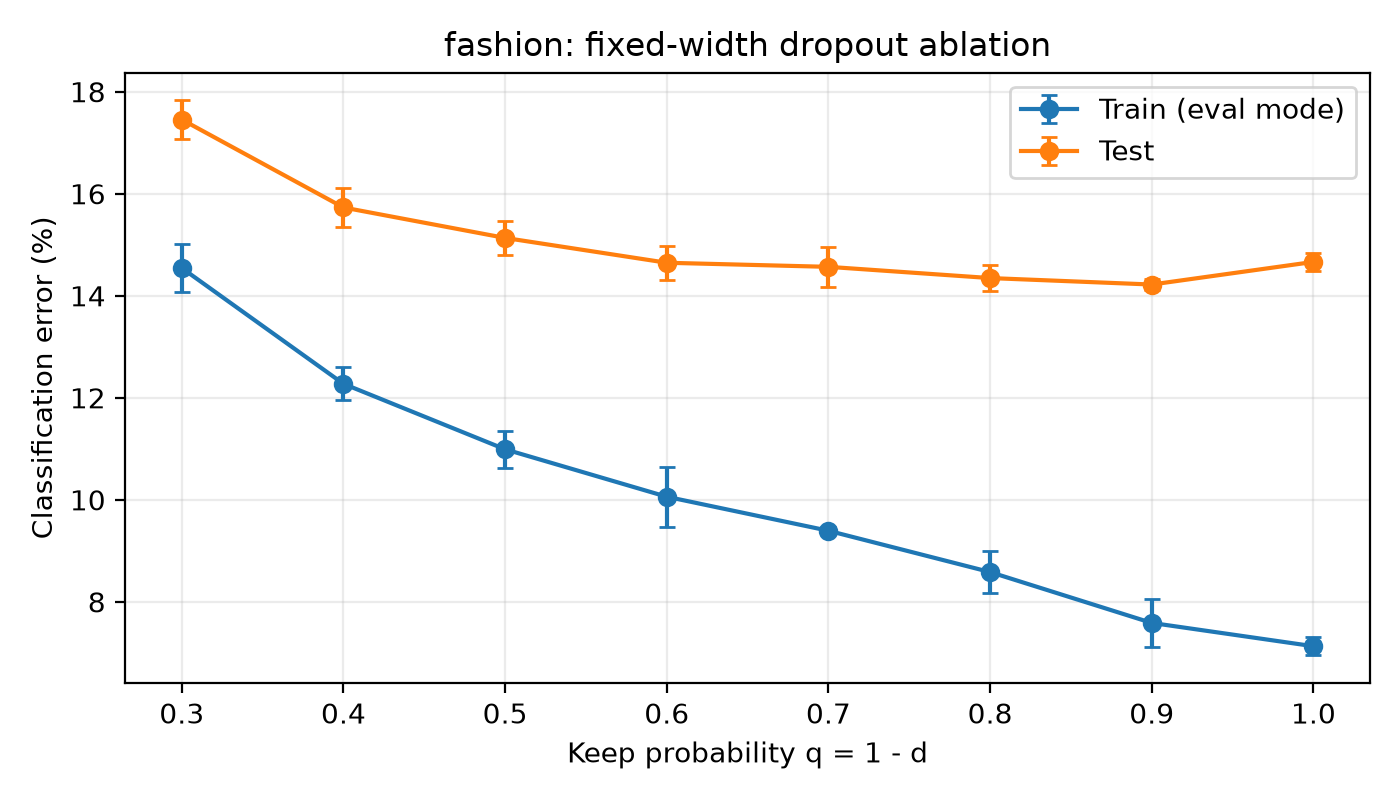
\includegraphics[width=0.78\linewidth]{figures/fashion_keep_probability.png}
\caption{Keep-probability ablation curve for Fashion-MNIST extension under protocol \texttt{dropout-24cs2032-v1}. Error increases monotonically for retention probabilities below $q = 0.8$ ($d > 0.2$).}
\label{fig:keep_prob_fashion}
\end{minipage}
\end{figure*}

The MNIST curve (Fig.~\ref{fig:keep_prob_mnist}) displays a distinct U-shaped profile. When $q=1.0$ (no dropout), overfitting leads to elevated test error ($4.320\%$). As $q$ decreases into the intermediate regime ($q \in [0.6, 0.9]$, corresponding to $d \in [0.1, 0.4]$), test error reaches an optimal trough between $3.820\%$ and $3.900\%$. However, when retention falls to $q \le 0.4$ ($d \ge 0.6$), test error rises steeply to $5.110\%$.

On Fashion-MNIST (Fig.~\ref{fig:keep_prob_fashion}), the optimal retention is higher ($q=0.8$, $d=0.2$). As retention probability decreases below $q=0.5$ ($d > 0.5$), performance degrades rapidly.

\section{Discussion and Comparison with Srivastava et al. (2014)}

\subsection{Comparison with Original Findings}
In Table~2 of Srivastava et al.~\cite{srivastava2014dropout}, the authors report a test error of $1.25\%$ for a standard feedforward neural network with dropout and ReLU activations on MNIST ($3 \times 1024$ hidden units, 60,000 training examples, SGD with momentum). In our reduced-scale reproduction, our baseline achieves $4.320 \pm 0.295\%$ and our validation-selected model achieves $3.843 \pm 0.282\%$.

Our reduced-scale experiment is not an apples-to-apples comparison with the original paper. As detailed below, these results reflect fundamentally different experimental budgets:
\begin{enumerate}
\item \textbf{Network Capacity:} Srivastava et al. evaluated networks with $3 \times 1024$ units (and up to $8{,}192$ units in wider experiments), whereas our model utilizes 256 units per hidden layer ($335{,}114$ total parameters).
\item \textbf{Dataset Scale:} The original paper utilized all 60,000 available training examples, compared to our subsampled set of 10,000 training examples.
\item \textbf{Training Budget and Optimization:} The original work trained networks for hundreds of epochs using Stochastic Gradient Descent (SGD) with momentum and max-norm constraints ($\|W\|_2 \le c$), whereas our experiment employs Adam for 20 epochs without weight constraints.
\item \textbf{Regularization Formulation:} We utilize modern inverted dropout during training rather than test-time weight rescaling.
\end{enumerate}

Despite these substantial budget differences, our experiments reproduce the fundamental qualitative finding of Srivastava et al. (Fig.~9(a)): generalization error exhibits a U-shaped dependence on retention probability, where intermediate keep probabilities offer optimal regularization and high dropout rates underfit under the fixed training budget. The Fashion-MNIST benchmark has no numerical counterpart in the 2014 paper and is evaluated strictly as an extension using the same experimental protocol.

\subsection{Differential Regularization Behavior}
A compelling finding of this study is the marked difference in optimal drop rate between MNIST ($d^* = 0.4$) and Fashion-MNIST ($d^* = 0.2$). MNIST digits consist of clean, high-contrast, stroke-based patterns with substantial redundant pixel information, making the representations highly amenable to aggressive unit deactivation. 

Conversely, Fashion-MNIST exhibits complex, subtle textures and fine-grained visual distinctions between apparel categories. High drop rates produced higher train and test error under the fixed 20-epoch budget, consistent with stronger underfitting for $d \ge 0.5$.

\section{Failure Analysis and Limitations}

\subsection{Empirical Failure Case Analysis}
To inspect the nature of model errors, we examined misclassified test examples from the validation-selected models across both datasets. Figure~\ref{fig:failures} displays representative test failure cases.

\begin{figure}[htbp]
\centering
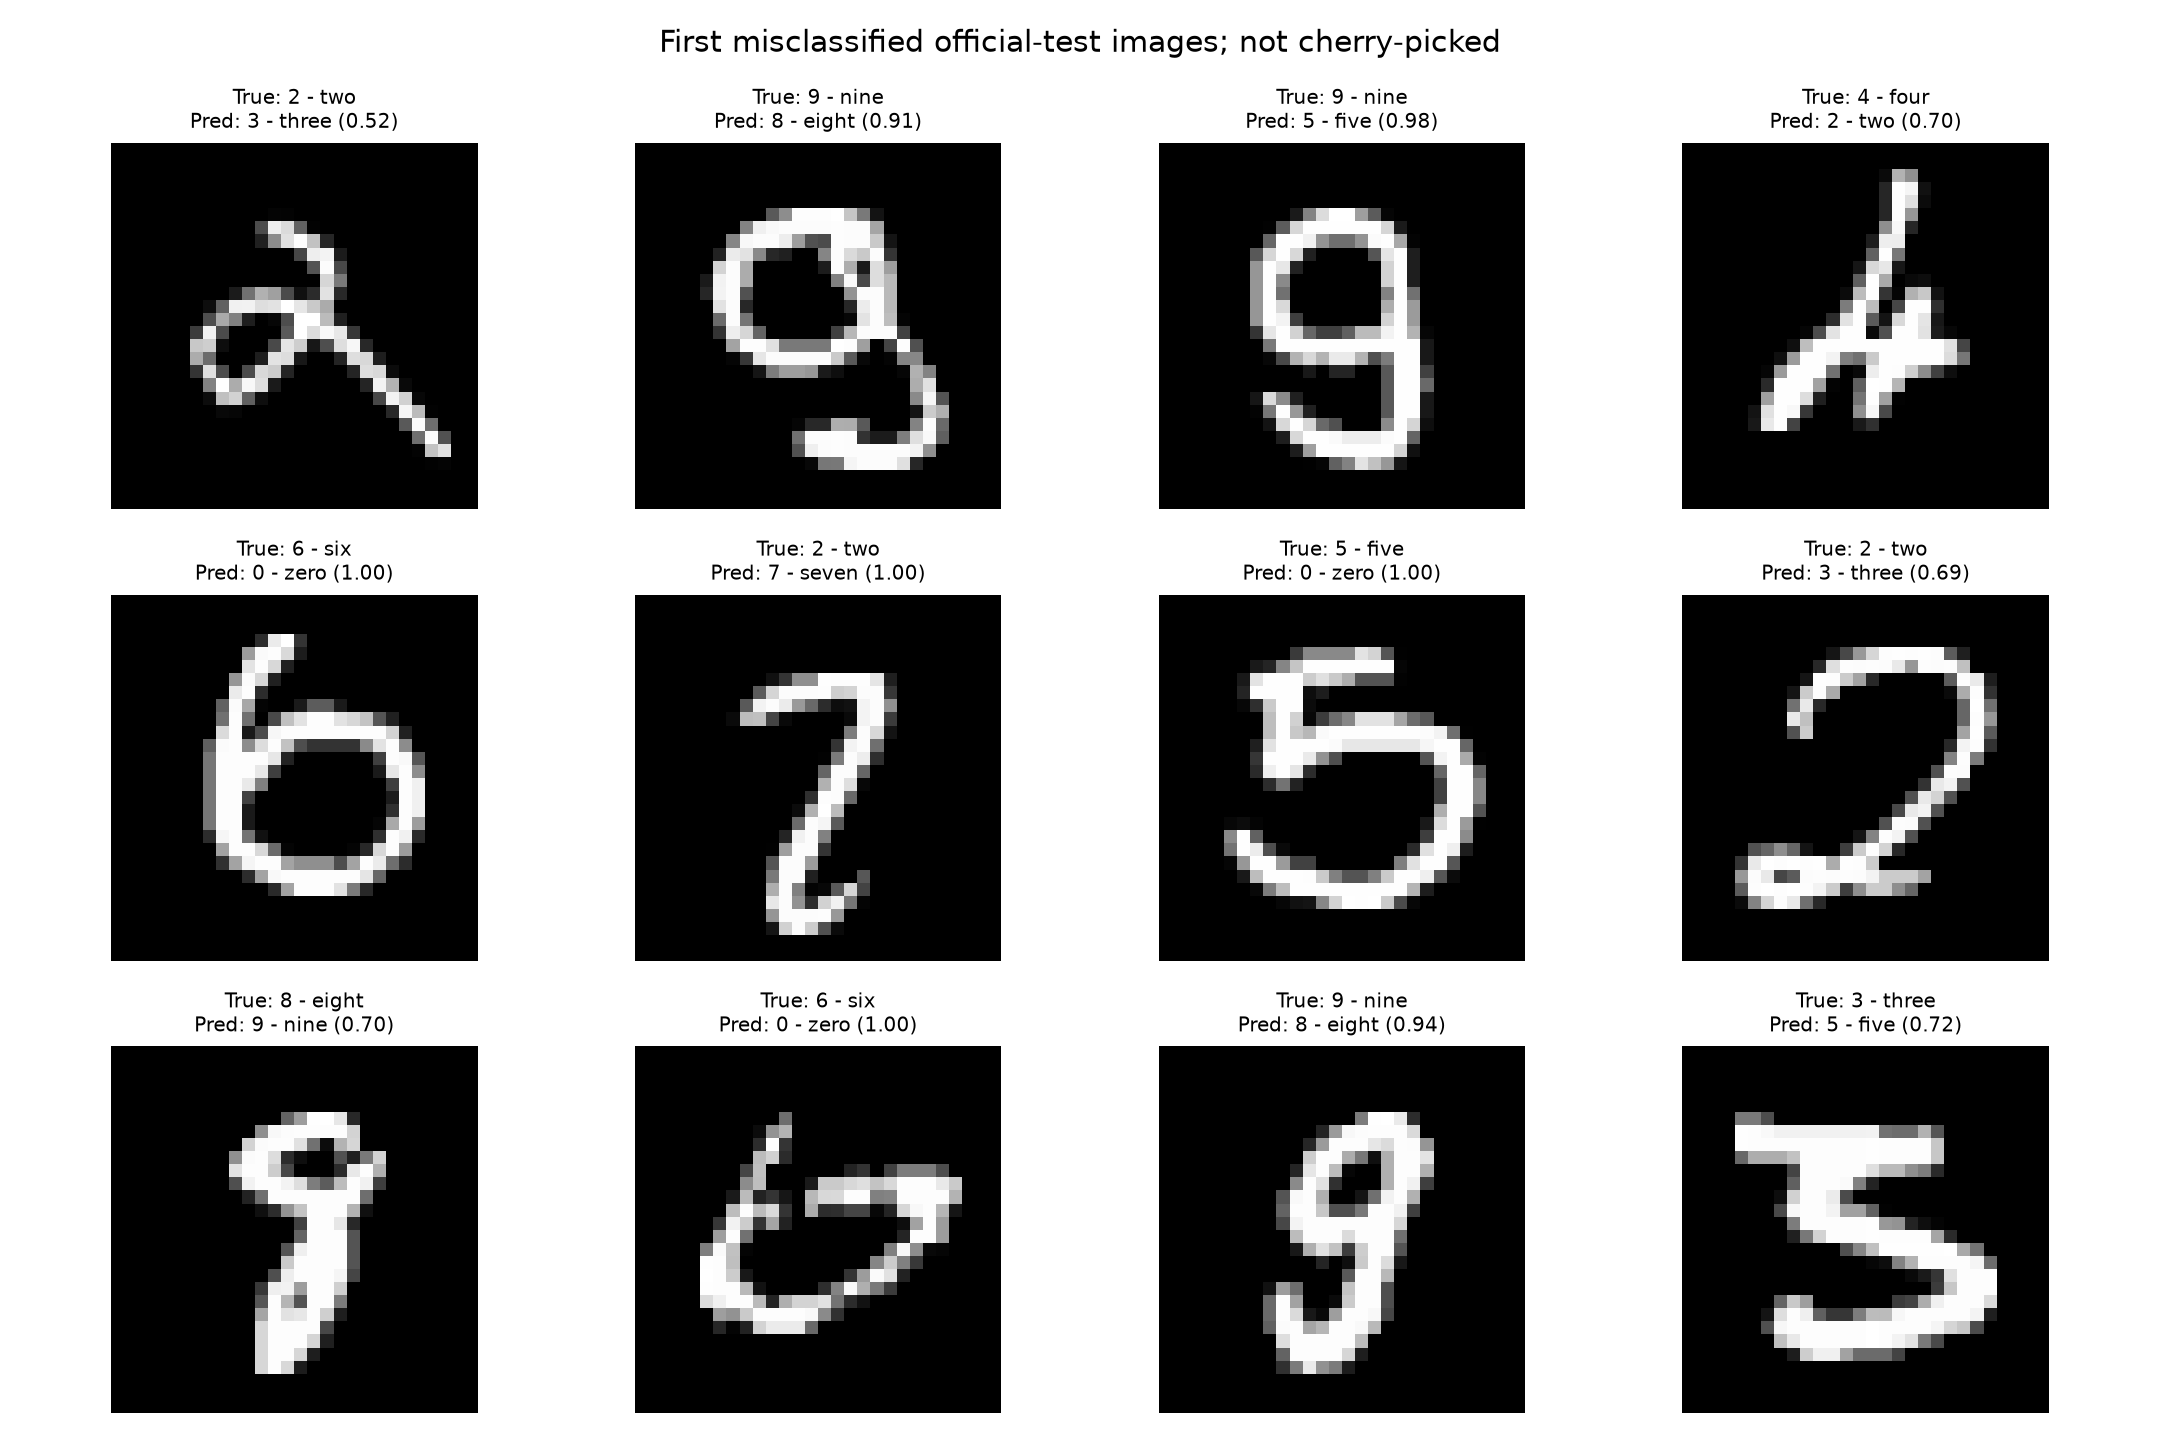
\includegraphics[width=0.45\columnwidth]{figures/mnist_failure_cases.png}
\hfill
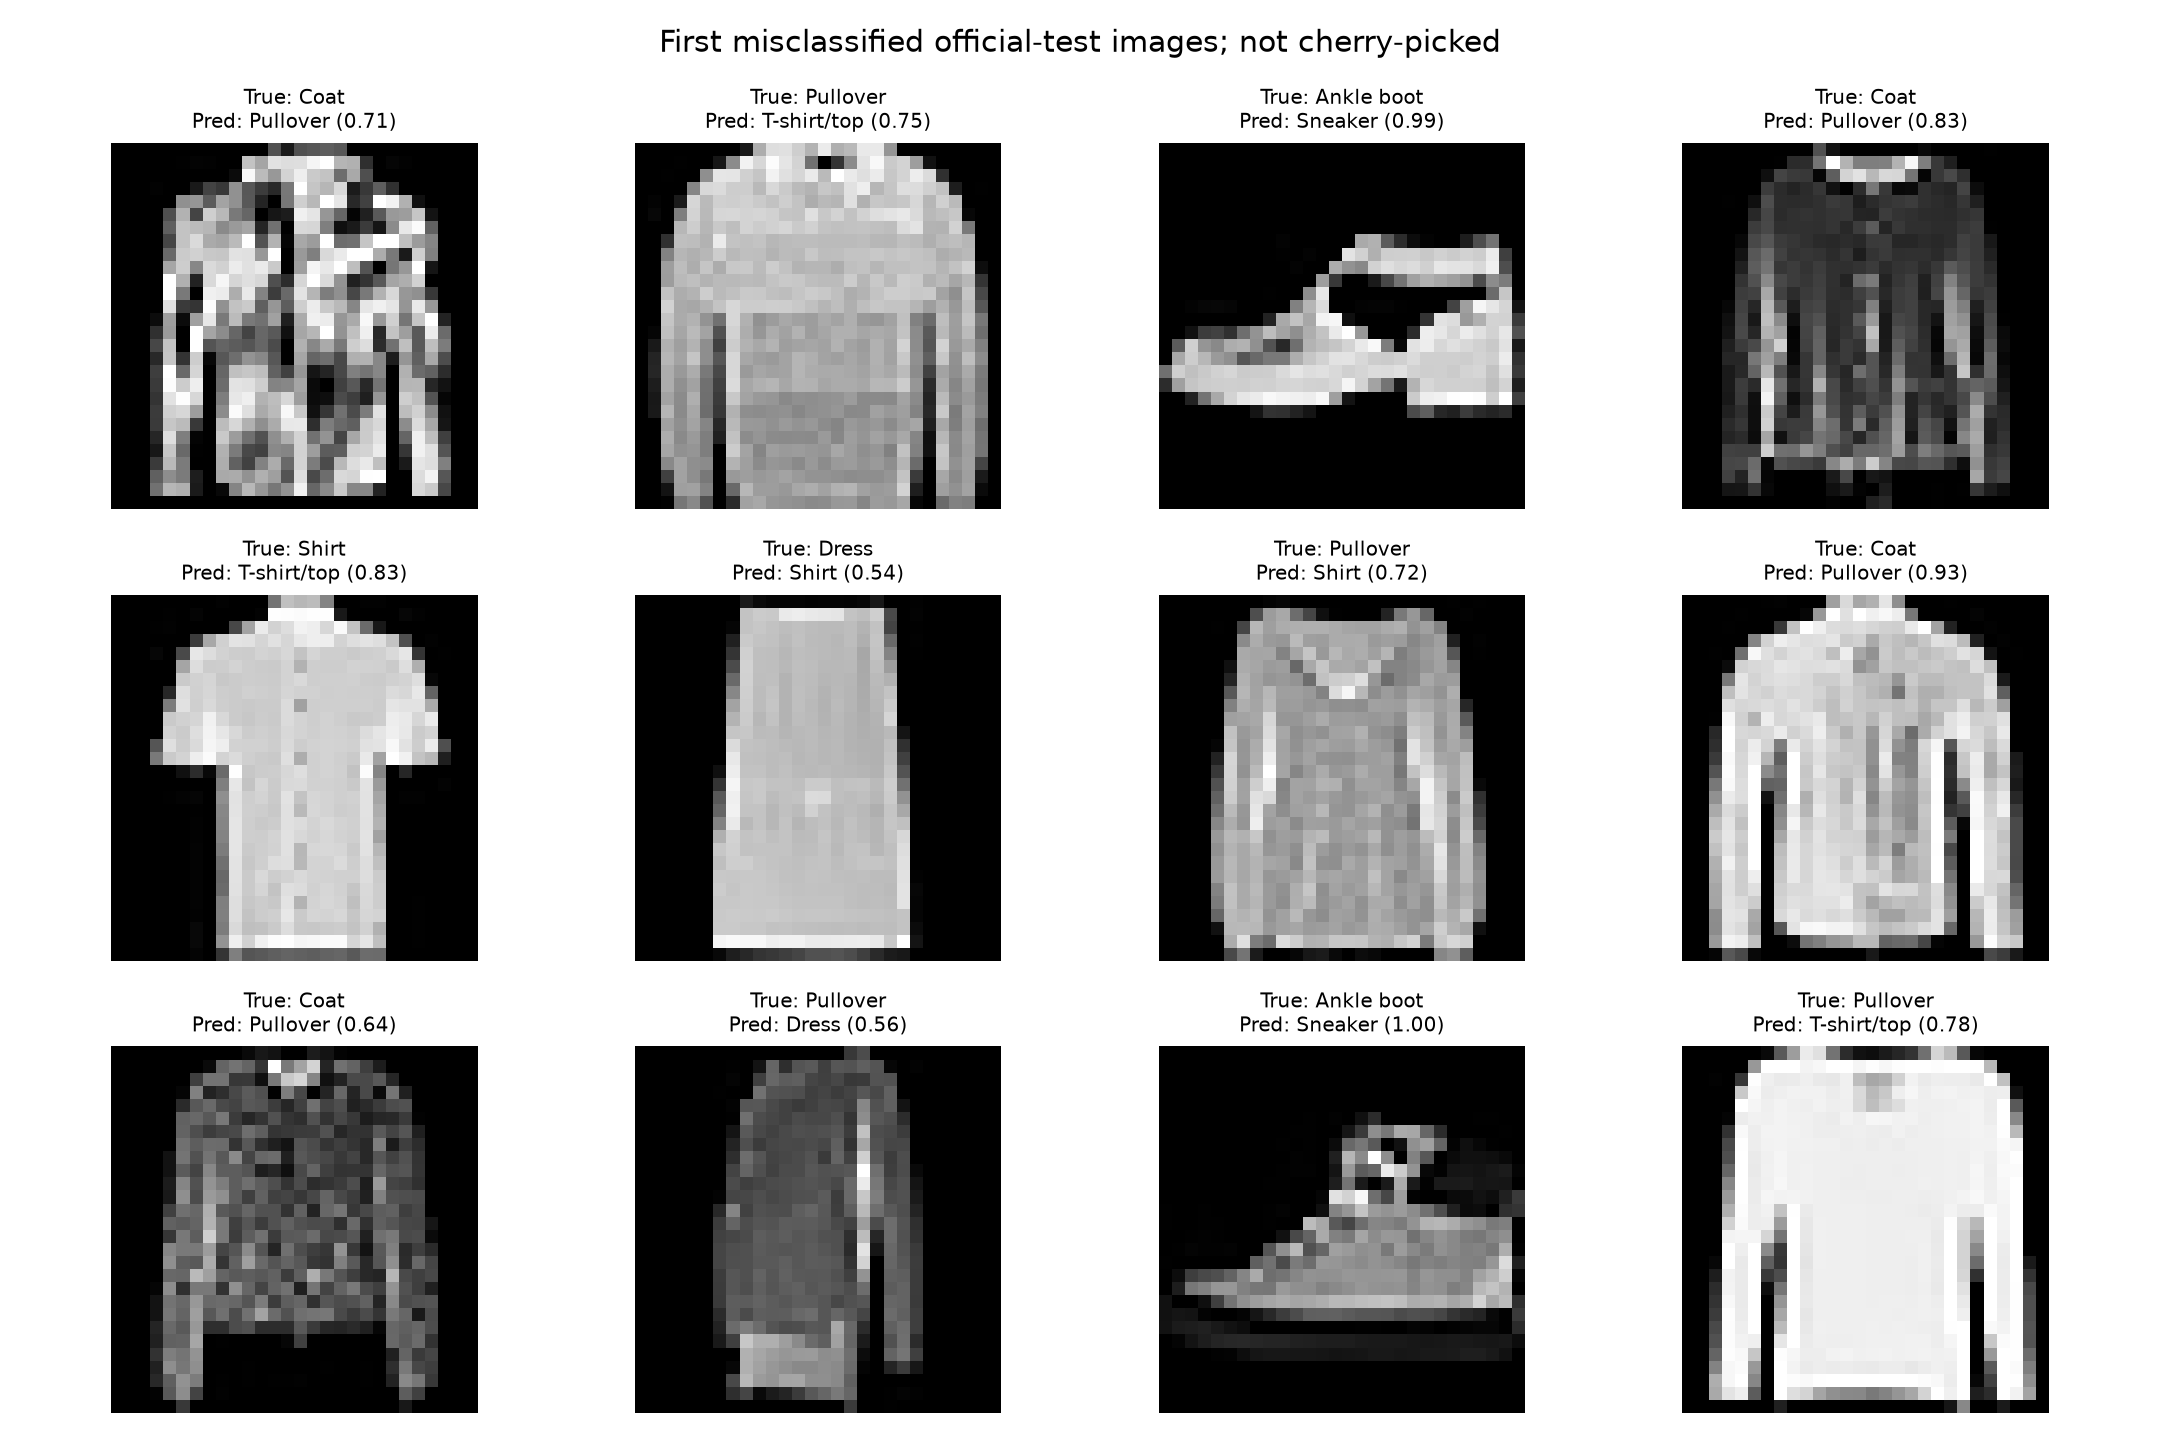
\includegraphics[width=0.45\columnwidth]{figures/fashion_failure_cases.png}
\caption{Representative misclassified test instances on MNIST ($d=0.4$, left) and Fashion-MNIST ($d=0.2$, right) showing true labels, model predictions, and softmax confidences.}
\label{fig:failures}
\end{figure}

On MNIST (Fig.~\ref{fig:failures}, left), typical errors involve ambiguous handwriting: a handwritten digit with true label 2 is classified as 3 with confidence 0.52, and a handwritten digit with true label 9 is classified as 8 with confidence 0.91. From visual inspection, the handwritten strokes in these instances visually resemble the predicted alternative classes.

On Fashion-MNIST (Fig.~\ref{fig:failures}, right), errors consistently concentrate at boundaries between semantically adjacent clothing categories: a true Coat is classified as Pullover with confidence 0.71, and a true Ankle Boot is classified as Sneaker with confidence 0.99. At $28 \times 28$ grayscale resolution, global silhouettes of coats and pullovers or boots and sneakers share a similar silhouette and may be confused under low resolution and small training budgets. Fully connected networks lack spatial inductive bias, rendering subtle texture distinctions challenging to resolve.

\subsection{Methodological Limitations}
We identify the following methodological constraints:
\begin{enumerate}\setlength{\itemsep}{0pt}\setlength{\parskip}{0pt}
\item \textbf{Seed Sample Size:} All results are evaluated over three random seeds ($42, 43, 44$). While reporting sample standard deviation with $ddof=1$ reflects variance, this sample size is insufficient for formal statistical significance testing.
\item \textbf{Fixed Training Budget:} All models were trained for exactly 20 epochs. High dropout rates inherently slow down convergence; allocating additional epochs might partially recover performance for $d \ge 0.5$.
\item \textbf{Subsampled Training Split:} Using 10,000 training examples magnifies regularizer sensitivity relative to the full 60,000 dataset.
\item \textbf{Verification Scope:} The results reported here were executed and verified locally on Apple Silicon CPU hardware. Hosted cloud execution (Google Colab) has not been verified.
\end{enumerate}

\section{Conclusion}
This study presented a complete, from-scratch implementation of inverted dropout in PyTorch, accompanied by an empirical ablation study across eight drop rates on MNIST and Fashion-MNIST. By strictly adhering to validation-based model selection, we demonstrated that moderate dropout rates reliably reduce test error relative to the unregularized baseline ($11.03\%$ relative reduction on MNIST at $d=0.4$; $2.16\%$ relative reduction on Fashion-MNIST at $d=0.2$). 

Crucially, our experiments also revealed negative results: canonical rates such as $d=0.5$ underperformed the baseline on Fashion-MNIST, and high drop rates ($d \ge 0.6$) degraded accuracy across both benchmarks. These findings corroborate the core regularization hypothesis of Srivastava et al. while confirming that dropout is not universally beneficial without systematic validation calibration.

\section*{Assistance and Provenance Statement}
Artificial intelligence tools (ChatGPT and Antigravity) were employed for implementation guidance, code review, local workflow automation, verification, and documentation formatting. All experimental results, figures, tables, and numerical metrics presented in this paper originate entirely from recorded real-data runs executed in this project repository and independently audited from persistent artifacts. External assistance is disclosed in accordance with course policy.

{\small
\bibliographystyle{IEEEtran}
\bibliography{references}
}

\end{document}
